%NOTE: COMPILE IN TERMINAL USING LUALATEX
\documentclass[a4paper,8pt]{standalone}

\usepackage{tikz-feynman}
%\usetikzlibrary{external}             %% Load the `external` library
%\tikzexternalize
%\immediate\write18{mkdir -p pgf-img}
%\tikzexternalize[                     %% Activate externalization
%  system call={                       %% Use lualatex in system call
%    lualatex \tikzexternalcheckshellescape -halt-on-error -interaction=batchmode -jobname="\image" "\texsource" || rm "\image.pdf"
%  },
%]

\begin{document}

%\feynmandiagram [horizontal=a to d]{
%    b -- [gluon] c -- [fermion,edge label'=$t$] c1 -- [gluon] b1,
%    c -- [fermion,edge label=$t$] a -- [fermion,edge label=$\bar t$] c1,
%    a -- [scalar,edge label=$H$] d,
%    b -- [opacity=0] b1,
%};

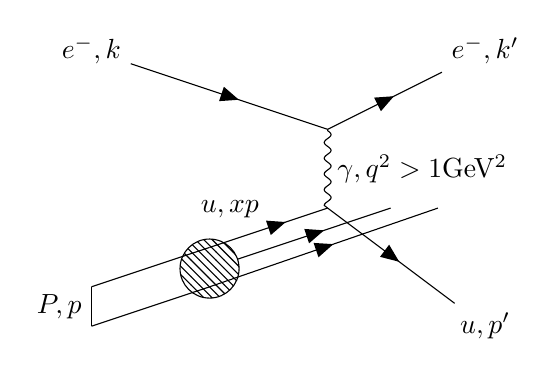
\begin{tikzpicture}
    \begin{feynman}
        \vertex (a1) {$e^-,k$};
        \vertex[right=5cm of a1] (a2) {$e^-,k'$};
        \vertex[below=3.5cm of a2] (a3) {$u,p'$};

        \vertex[below=3cm of a1] (b1);
        \vertex[below=0.5cm of b1] (b2);
        \vertex at ($(b1)+(1.5cm,0cm)$) (b3);
        \vertex at ($(b1)+(1.5cm,0.5cm)$) (b5);
        \vertex[above=-0.15cm of b3,blob] (b4) {};

        \vertex at ($(a1)+(3cm,-1cm)$) (c1);
        \vertex[below=1cm of c1] (c2);
        \vertex[right=0.8cm of c2] (c3);
        \vertex[right=1.4cm of c2] (c4);

        \diagram* {
            (a1) -- [fermion] (c1) -- [fermion] (a2),
            (c1) -- [photon,edge label={$\gamma,q^2>1$GeV$^2$}] (c2),
            (c2) -- [anti fermion,edge label'={$u,xp$}] (b5) -- (b1) -- [plain,edge label'={$P,p$}] (b2) -- (b3),
            (b4) --  [fermion] (c3),
            (b3) -- [fermion] (c4),
            (c2) -- [fermion] (a3),
        };
    \end{feynman}
\end{tikzpicture}


\end{document}
